% =============================================================================

\begin{figure}
\centering
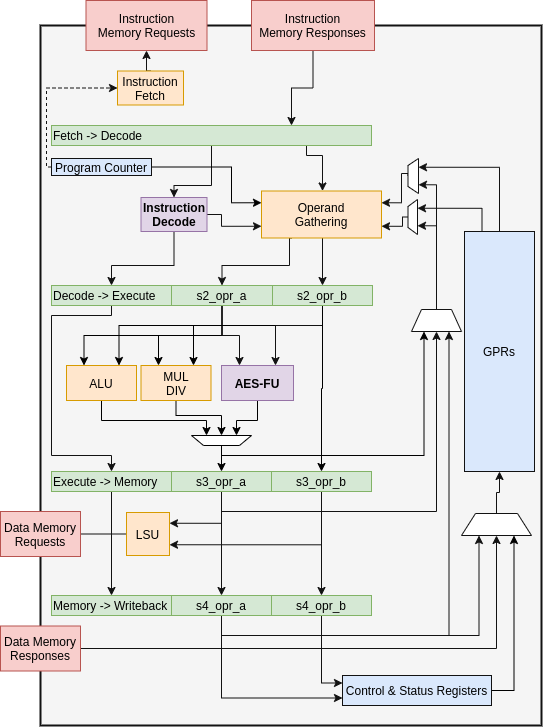
\includegraphics[scale=0.45,angle=90]{diagrams/scarv-cpu-uarch.png}
\caption{Core $2$: \CORE{2}.}
\label{fig:design:cpu_block:2}
\end{figure}

% -----------------------------------------------------------------------------

The evaluation of each ISE considers two different RISC-V compliant base
micro-architectures, which constitute two different host cores:

\begin{itemize}
\item The \CORE{2}\footnote{%
        \ifbool{anonymous}{Details of this core have been anonymised to comply with the TCHES submission guidelines.}{\url{https://github.com/scarv/scarv}}
      } core 
      supports the 
      RV32IMC 
      instruction set, i.e.,
      the 
             $32$-bit~\cite[Section 2]{RV:ISA:I:19} 
      base integer ISA plus 
      standard M~\cite[Section  7]{RV:ISA:I:19}
               (or   multiply)
               and
               C~\cite[Section 16]{RV:ISA:I:19}
               (or compressed)
               extensions.
      Per the block diagram shown in~\REFFIG{fig:design:cpu_block:2},
      the core 
      executes instructions using a $5$-stage, in-order pipeline;
      no mechanism for
      branch prediction
      is supported.
      Although there are two memory interfaces, one for (instruction) fetch and one for (data) memory access stages,
      no
      instruction or data caches 
      are supported.
      The core implements various performance counters,
      and
      elements of the
      RISC-V Privileged Resource Architecture (PRA)~\cite[Chapter 3]{RV:ISA:II:17}
      related to exception and interrupt handling.

\item The \CORE{1}~\cite{rocket:16} 
        core
      executes instructions using a $5$-stage, in-order pipeline
      which is highly configurable.
      We take advantage of this, considering two variants whose configuration
      is outlined in
      \REFFIG{fig:rocket:32} 
      and 
      \REFFIG{fig:rocket:64}:
      the variants represent single $32$-bit and $64$-bit cores respectively,
      and so
      support  the 
      RV32IMC 
      instruction set, i.e.,
      the 
             $32$-bit~\cite[Section 2]{RV:ISA:I:19} 
      (resp. $64$-bit~\cite[Section 5]{RV:ISA:I:19})
      base integer ISA plus 
      standard M~\cite[Section  7]{RV:ISA:I:19}
               (or   multiply)
               and
               C~\cite[Section 16]{RV:ISA:I:19}
               (or compressed)
               extensions.
      Each varient is configured to support
      an instruction cache, 
      a  data        cache,
      and
      a  branch prediction mechanism,
      but 
      no floating-point support.

\end{itemize}

\noindent
To support a given ISE, two modifications were made to each host core:
1) the instruction decoder was modified to support identification and 
   operand selection for instructions in the ISE,
   and
2) an AES Functional Unit (AES-FU) was added to support execution of
   (i.e., ISE-specific computation by) those instructions:
   the \CORE{2} core integrates the AES-FU directly into the pipeline,
   whereas
   the \CORE{1} core accesses   the AES-FU via the
   Rocket Custom Coprocessor (RoCC)~\cite[Section 4]{rocket:16}
   interface.
Due to \REFREQ{req:2}, 
specifically that each instruction uses at most $2$ source and $1$ destination register, 
neither micro-architecture required further structural alteration, so
a synthesis-time parameter was sufficient to switch between different 
ISEs.

% =============================================================================
